\chapter{Introduction}

In algebraic topology, the fundamental group\footnote{Henri Poincare} is a mathematical group associated to any given pointed topological space that provides a way to determine when two paths, starting and ending at a fixed base point, can be continuously deformed into each other. It records information about the basic shape, or holes, of the topological space. The fundamental group is a topological invariant: homeomorphic topological spaces have isomorphic (the same except name) fundamental group.\\
In order to understand the fundamental group, we need to know some concepts from set theory, group theory and topology. So, we shall review.
\section{Basic Set Theory}
Without set theory it is impossible to study group theory and topology. Of course it is impossible to study mathematics without set theory, as it is the foundation. So let's start to review set theory by giving the intuitive definition of what a set mean.
\begin{definition}
Any well defined collection of object is called a set.
\end{definition}
The objects comprising the set are called its elements or members.
\begin{definition}
A set $A$ is said to be a subset of $B$ or equivalently, $B$ is a superset of $A$, written
$$ A\subset B ~or~ B\supset A$$
iff each elements in $A$ belongs to $B$.
\end{definition}

\begin{definition}[\textbf{Equality}]
Two sets $A$ and $B$ are equal if and only if  $A\subset B$ and $B\subset A$.
\end{definition}
We always use the above definition to prove two sets are equal.
\begin{definition}
A set with no elements in it is called the \textbf{empty set} and  it is denoted by $\emptyset$.
\end{definition}

\begin{remark}
The empty set is a subset of every set.
\end{remark}
\begin{definition}
The \textbf{union} of two sets $A$ and $B$ is defined as
\[
A \cup B = \{x : x \in A \text{ or } x \in B \};
\]
\end{definition}
\begin{definition}
The \textbf{intersection} of $A$ and $B$  is defined by
\[
A \cap B = \{x :  x \in A \text{ and } x \in B \}.
\]
\end{definition}
We can consider a finite union and intersection of more than two sets.  In this case we write
\[
\bigcup_{i = 1}^{n} A_{i} = A_{1} \cup \ldots \cup A_n
\]
and
\[
\bigcap_{i = 1}^{n} A_{i} = A_{1} \cap \ldots \cap A_n
\]
for the union and intersection, respectively, of the sets $A_1, \ldots, A_n$.
\begin{definition}
When two sets have no elements in common, they are said to be \textbf{disjoint}. Two sets $A$ and $B$ are disjoint exactly when $A \cap B = \emptyset$.
\end{definition}
Sometimes we will work within one fixed set $U$, called the \textbf{universal set}.  For any set $A \subset U$, we define the \textbf{complement} of $A$, denoted by $A'$, to be the set
\[
A' = \{ x : x \in U \text{ and } x \notin A \}.
\]
The \textbf{difference} of two sets $A$ and $B$ is defined by
\[
A \setminus B = A \cap B'  = \{ x : x \in A \text{ and } x \notin B \}.
\]

\begin{proposition}
Let $A$, $B$, and $C$ be sets. Then
\begin{enumerate}

\rm\item\it
$A \cup A = A$, $A \cap A = A$, and $A \setminus A = \emptyset$;

\rm\item\it
$A \cup \emptyset = A$ and $A \cap \emptyset = \emptyset$;

\rm\item\it
$A \cup (B \cup C) = (A \cup B) \cup C$ and  $A \cap (B \cap C) = (A \cap B) \cap C$;

\rm\item\it
$A \cup B = B \cup A$ and $A \cap B = B \cap A$;

\rm\item\it
$A \cup (B \cap C) = (A \cup B) \cap (A \cup C)$;

\rm\item\it
$A \cap (B \cup C) = (A \cap B) \cup (A \cap C)$.

\end{enumerate}
\end{proposition}
The following theorem is a very important theorem in set theory due to British mathematician Augustus De Morgan.
\begin{theorem}[\textbf{De Morgan's Laws}]
Let $A$ and $B$ be sets. Then
\begin{enumerate}

\rm\item\it
$(A \cup B)' = A' \cap B'$;

\rm\item\it
$(A \cap B)' = A' \cup B'$.

\end{enumerate}
\end{theorem}
\begin{proof}
(1)
We must show that $(A \cup B)' \subset A' \cap B'$ and $(A \cup B)' \supset A' \cap B'$. Let $x \in (A \cup B)'$.  Then $x \notin A \cup B$. So $x$ is neither in $A$ nor in $B$, by the definition of the union of sets.  By the definition of the complement, $x \in A'$ and $x \in B'$.  Therefore, $x \in A' \cap B'$ and we have $(A \cup B)' \subset A' \cap B'$.

To show the reverse inclusion, suppose that $x \in A' \cap B'$.  Then $x \in A'$ and $x \in B'$, and so $x \notin A$ and $x \notin B$.  Thus $x \notin A \cup B$ and so $x \in (A \cup B)'$.  Hence, $(A \cup B)' \supset A' \cap B'$ and so $(A \cup B)' = A' \cap B'$.

The proof of (2) is similar.
\end{proof}

\begin{definition}
Given sets $A$ and $B$, we can define a new set $A \times B$, called the \textbf{Cartesian product}\footnote{Rene Descartes} of $A$ and $B$, as a set of ordered pairs.  That is,
$$
A \times B = \{ (a,b) : a \in A \text{ and } b \in B \}.
$$
\end{definition}

If $A = A_1 = A_2 = \cdots = A_n$, we often write $A^n$ for $A \times \cdots \times A$ (where $A$ would be written $n$ times).   For example, the set ${\mathbb R}^3$ consists of all of 3-tuples of real numbers.
\begin{definition}
Subsets of $A \times B$ are called \textbf{relations}.
\end{definition}
\begin{definition}
A \textbf{mapping} or \textbf{function} $f \subset A \times B$ from a set $A$ to a set $B$ to be the special type of  relation in which for each element $a \in A$ there is a unique element $b \in B$ such that $(a, b) \in f$; that means for every element in $A$, $f$ assigns a unique element in $B$.  We usually write $f:A \rightarrow B$ or $A \stackrel{f}{\rightarrow} B$.  Instead of writing down ordered pairs  $(a,b) \in A \times B$, we write $f(a) = b$ or $f : a \mapsto b$.  The set  $A$ is called the \textbf{domain} of $f$ and
\[
f(A) = \{ f(a) : a \in A \} \subset B
\]
is called the \textbf{range} or \textbf{image} of $f$.
\end{definition}
We can think of the elements in the function's domain as input values and the elements in the function's range as output values.

A relation cannot be a mapping because it is not well-defined. A relation is \textbf{well-defined} if each element in the domain is assigned to a \textbf{unique} element in the range.

If $f:A \rightarrow B$ is a map and the image of $f$ is $B$, i.e., $f(A) = B$, then $f$ is said to be \textbf{onto} or \textbf{surjective}. In other words, if there exists an $a \in A$ for each $b \in B$ such that $f(a) = b$, then $f$ is onto. A map is \textbf{one-to-one} or \textbf{injective} if $a_1 \neq a_2$ implies $f(a_1) \neq f(a_2)$.  Equivalently, a function is one-to-one if $f(a_1) = f(a_2)$ implies $a_1 = a_2$.  A map that is both one-to-one and onto is called \textbf{bijective}.

\begin{proposition}
Let $f : A \rightarrow B$, $g : B \rightarrow C$, and $h : C \rightarrow D$. Then
\begin{enumerate}

\rm\item\it
The composition of mappings is associative; that is, $(h \circ g) \circ f = h \circ (g \circ f)$;

\rm\item\it
If $f$ and $g$ are both one-to-one, then the mapping $g \circ f$ is one-to-one;

\rm\item\it
If $f$ and $g$ are both onto, then the mapping $g \circ f$ is onto;

\rm\item\it
If $f$ and $g$ are bijective, then so is $g \circ f$.

\end{enumerate}
\end{proposition}

If $S$ is any set, we will use $id_S$ or $id$ to denote the \textbf{identity mapping} from $S$ to itself.  Define this map by $id(s) = s$ for all $s \in S$.  A map $g: B \rightarrow A$ is an \textbf{inverse mapping} of $f: A \rightarrow B$ if $g \circ f = id_A$ and $f \circ g = id_B$; in other words, the inverse function of a function simply "undoes" the function.   A map is said to be \textbf{invertible} if it has an inverse.  We usually write $f^{-1}$ for the inverse of $f$.


\begin{theorem}
A mapping is invertible if and only if it is both one-to-one and onto.
\end{theorem}

\begin{proof}
Suppose first that $f:A \rightarrow B$ is invertible with inverse $g: B \rightarrow A$. Then $g \circ f = id_A$ is the identity map; that is, $g(f(a)) = a$. If $a_1, a_2 \in A$ with $f(a_1) = f(a_2)$, then $a_1 = g(f(a_1)) = g(f(a_2)) = a_2$.  Consequently, $f$ is one-to-one.  Now suppose that $b \in B$. To show that $f$ is onto, it is necessary to find an $a \in A$ such that $f(a) = b$, but $f(g(b)) = b$ with $g(b) \in A$. Let $a = g(b)$.

Now assume the converse; that is, let $f$ be bijective.  Let $b \in B$.  Since $f$ is onto, there exists an $a \in A$ such that $f(a) = b$.  Because $f$ is one-to-one, $a$ must be unique. Define $g$ by letting $g(b) = a$.  We have now constructed the inverse of $f$.
\end{proof}

The review that we have seen so far is just to define an equivalence relation. It is the most important concept in this section that we need for our understanding of the fundamental group.

\begin{definition}
An \textbf{equivalence relation} on a set $X$ is a relation $R \subset X \times X$ such that
\begin{description}
  \item[Reflexive:] $(x, x) \in R$ for all $x \in X$.
  \item[Symmetric:] $(x, y) \in R$ implies $(y, x) \in R$.
  \item[Transitive:] $(x, y)$ and $(y, z) \in R$ imply $(x, z) \in R$.
\end{description}
\end{definition}

A \textbf{partition} ${\mathcal P}$ of a set $X$ is a collection of nonempty sets $X_1, X_2, \ldots$ such that $X_i \cap X_j = \emptyset$ for $i  \neq j$ and $\bigcup_k X_k = X$. Let $\sim$ be an equivalence relation on a set $X$ and let $x \in X$.  Then $[x] = \{ y \in X : y \sim x \}$ is called the \textbf{equivalence class} of $x$.

The important thing about an equivalence relation is that it gives rise to a partition via equivalence classes.  Also, whenever a partition of a set exists, there is some natural  underlying equivalence relation, as the following theorem demonstrates.

\medskip

\begin{theorem}
Given an equivalence relation $\sim$ on a set $X$, the equivalence classes of $X$ form a partition of $X$.  Conversely, if ${\mathcal P} = \{ X_i\}$ is a partition of a set $X$, then there is an equivalence relation on $X$ with equivalence classes $X_i$.
\end{theorem}

\begin{proof}
Suppose there exists an equivalence relation $\sim$ on the set $X$.  For any $x \in X$, the reflexive property shows that $x \in [x]$ and so $[x]$ is nonempty.  Clearly $X = \bigcup_{x \in X} [x]$.  Now let $x, y \in X$. We need to show that either $[x] = [y]$ or $[x] \cap [y] = \emptyset$.  Suppose that the intersection of $[x]$ and $[y]$ is not empty and that $z \in [x] \cap [y]$. Then $z \sim x$ and $z \sim y$.  By symmetry and transitivity $x \sim y$; hence, $[x] \subset [y]$.  Similarly, $[y] \subset [x]$ and so $[x] = [y]$.  Therefore, any two equivalence classes are either disjoint or exactly the same.

Conversely, suppose that ${\mathcal P} = \{X_i\}$ is a partition of a set $X$.  Let two elements be equivalent if they are in the same partition. Since $x\sim x$, the relation is reflexive.  If $x$ is in the same partition as $y$, then $y$ is in the same partition as $x$, so $x \sim y$ implies $y \sim x$.  Finally, if $x$ is in the same partition as $y$ and $y$ is in the same partition as $z$, then $x$ must be in the same partition as $z$, and transitivity holds.
\end{proof}
\newpage
\section{Basic Group Theory}
As we have mentioned in the abstract our aim is to understand the fundamental group. So, what is the fundamental group? Well, it is a mathematical group. What is a mathematical group? To answer this question and to see some basic results which are very helpful for our understanding of the fundamental group  we are forced to review group theory. We begin our revision by defining a Group in mathematics.

\begin{definition}[\textbf{Group}]
An algebraic structure with one binary operation $(G,\Delta)$ is called a group iff\footnote{For definition if and iff are the same} the following four conditions are satisfied
\begin{enumerate}
  \item $\forall a,b\in G \Rightarrow a\Delta b \in G \qquad \qquad \text{Closure}$
  \item $\forall a,b,c \in G \Rightarrow a\Delta (b\Delta c)=(a\Delta b)\Delta c\qquad \text{Associative}$
  \item $\exists e\in G \ni  a\Delta e=e\Delta a \qquad \forall a \in G\qquad \text{Identity}$
  \item $\forall a\in G ,\exists a^{-1}\in G \ni a\Delta a^{-1} =e=a^{-1}\Delta a \qquad \text{Inverse}$
\end{enumerate}
\end{definition}Moreover if $\Delta$ is commutative the group $G$ is called an \textbf{abelian group}.\\
The above four conditions are called group axioms. In our definition of a mathematical group there is a word "algebraic structure". Algebraic structure is nothing but a non empty set together with one or more finitary operations defined on it. Hence we can rewrite our definition of a mathematical group as \textit{a non empty set with one binary operation defined on it.} From now on we designate $a\Delta b$ by $ab$.
\begin{example}
Here are some examples of groups.
\begin{itemize}
  \item  $(\mathbb{Z},+)$ The set of integers with addition is a group.
  \item $(\mathbb{Q},+)$ The set of rational numbers with addition is a group.
  \item $(\mathbb{C}^\times,\times)$ The set of non zero complex numbers with the usual multiplication is a group.
\end{itemize}
\end{example}
\begin{conj}
There exists a group structure in the set of prime numbers.
\end{conj}

\begin{lemma}\label{uniquee}
The identity element in a group is unique.
\end{lemma}
\begin{proof}
Suppose that $e$ and $e'$ are both identities in $G$. Then $eg = ge =g$ and $e'g = ge' = g$ for all $g \in G$. We need to show that $e =e'$. If we think of $e$ as the identity, then $ee' = e'$; but if $e'$ is the identity, then $ee' = e$. Combining these two equations, we have $e = ee' = e'$.
\end{proof}

\begin{lem}[\textbf{Cancellation Law}]\label{cancelem}
If $G$ is a group and $a, b, c \in G$, then $ba = ca$ implies $b = c$
and $ab = ac$ implies $b = c$.
\end{lem}
\begin{proof}
Multiplying the equations by the appropriate inverse gives us the desired result.
\end{proof}

\begin{lemma}\label{uniquei}
If $g$ is any element in a group $G$, then the inverse of $g$, $g^{-1}$, is unique.
\end{lemma}
\begin{proof}
Suppose $g'$ and $g''$ are inverses of $g\in G$. WTS $g'=g''$. Now, since $g'$ is the inverse of $g$ we have $gg'=e$ and we have $gg''=e$ as $g''$ is the inverse of $g$. From the uniqueness of the identity element in a group we conclude that $gg'=gg''$. Hence $g'=g''$ by lemma (\ref{cancelem}).
\end{proof}
\begin{remark}
We denote the unique inverse of $g$ by $g'$.
\end{remark}

\begin{proposition}[\textbf{Socks Shoe}]
Let $G$ be a group. If $a, b \in G$, then $(ab)^{-1} = b^{-1}a^{-1}$.
\end{proposition}


\begin{proof}
Let $a, b \in G$. Then $abb^{-1}a^{-1} = aea^{-1} = aa^{-1} = e$. Similarly, $b^{-1}a^{-1}ab = e$. But by lemma (\ref{uniquei}), inverses are unique; hence, $(ab)^{-1} = b^{- 1}a^{-1}$.
\end{proof}


\begin{proposition}
Let $G$ be a group.  For any $a \in G$, $(a^{-1})^{-1} = a$.
\end{proposition}


\begin{proof}
Observe that $a^{-1} (a^{-1})^{-1} = e$. Consequently, multiplying
both sides of this equation by $a$, we have
$$ (a^{-1})^{-1} = e (a^{-1})^{-1} = a a^{-1} (a^{-1})^{-1} = ae = a.$$
\end{proof}
It makes sense to write equations with group elements and group operations. If $a$ and $b$ are two elements in a group $G$, does there exist an element $x \in G$ such that $ax = b$? If such an $x$ does exist, is it unique? The following proposition answers both of these questions.


\begin{proposition}\label{group_equations}
Let $G$ be a group and $a$ and $b$ be any two elements in $G$. Then the equations $ax = b$ and $xa = b$ have unique solutions in $G$.
\end{proposition}


\begin{proof}
Suppose that $ax = b$. We must show that such an $x$ exists. Multiplying both sides of $ax = b$ by $a^{-1}$, we have $x = ex = a^{-1}ax = a^{-1}b$.


To show uniqueness, suppose that $x_1$ and $x_2$ are both solutions of $ax = b$; then $ax_1 = b = ax_2$. So $x_1 = a^{-1}ax_1 = a^{-1}ax_2 = x_2$. The proof for the existence and uniqueness of the solution of $xa = b$ is similar.
\end{proof}

\begin{definition}[\textbf{Subgroup}]
Let G be a group and $\emptyset \neq H\subset G$ we say that $H$ is a subgroup of $G$ if $H$ by itself is a group.
We denote $H$ a subgroup of $G$ by $H\lesssim G$.
\end{definition}

\begin{example}
Let $H=\{ \pm1,\pm i\}$, then $H$ with the usual multiplication $(H,\times)$ is a subgroup of $(\mathbb{C^{\times}},\times)$.
\end{example}
\begin{proposition}[\textbf{Subgroup test}]\label{subtest}
Let G be a group and $\emptyset \neq H\subset G$ we say that $H$ is a subgroup of $G$ iff
\begin{enumerate}
  \item $\forall a,b\in H \Rightarrow a\Delta b \in H \qquad \qquad \text{Closure}$
  \item $\forall a \in H,\exists a^{-1}\in H \ni a\Delta a^{-1} =e=a^{-1}\Delta a \qquad \text{Inverse}$
\end{enumerate}
\end{proposition}

\begin{definition}[\textbf{Normal Subgroup}]
A subgroup $N$ of a group $G$ is \textbf{normal} in G if $gN =Ng$ for all $g \in G$. We denote $N$ is a normal subgroup of $G$ by $N\lhd G$.
\end{definition}

\begin{remark}
$H$ is normal in $G$ doesn't mean $ah=ha$ for $a\in G$ and $h\in H$. This is not what normality mean; rather, it means if $a\in G$ and $h\in H$, then there exists elements $h'$ and $h''$ in $H$ such that $ah=h'a$ and $ha=ah''$.
\end{remark}
\begin{proposition}
A subgroup $H$ of $G$ is normal in $G$ iff $xHx^{-1}\subset H$ for all $x\in G$.
\end{proposition}
\begin{proof}
If $H$ is normal in $G$, then for any $x\in G$ and $h\in H$ there is $h'\in H$ such that $xh=h'x.$ Thus, $h'=xhx^{-1}$ and therefore $xHx^{-1}\subset H$.\\
Conversely, if $xHx^{-1}\subset H$ for all $x\in G$, then letting $x=a$, we have $aHa^{-1}\subset H$ or $aH\subset Ha$. On the other hand, letting $x=a^{-1}$ we have $a^{-1}H(a^{-1})^{-1}=a^{-1}Ha\subset H$ or $Ha\subset aH.$
\end{proof}
\begin{definition}[\textbf{Cosets}]
Let $G$ be a group and $H$ a subgroup of $G$.  We define a \textbf{left  coset} of $H$ with \textbf{representative} $g \in G$ to be the set $gH = \{ gh : h \in H \}.$ \textbf{Right cosets} can be defined similarly by $Hg = \{ hg : h \in H \}.$
\end{definition}
If left and right cosets coincide or if it is clear from the context to which type of coset that we are referring, we will use the word \textbf{coset} without specifying left or right.
\begin{lemma}\label{coslemma}
 $aH = bH$ if and only if $a \in bH$.
\end{lemma}
\begin{proof}
 If $aH=bH$, then $a = ae \in aH=bH$. Conversely, if $a \in bH$ we have $a = bh$ where $h \in H$, and therefore $aH = (bh)H = b(hH) = bH$.
\end{proof}

The coset of a group partitions the group as the following proposition demonstrates.
\newpage
\begin{proposition}
Let $H$ be a subgroup of a group $G$.  Then the left cosets of $H$ in $G$ partition $G$.  That is, the group $G$ is the disjoint union of the left cosets of $H$ in $G$.
\end{proposition}

\begin{proof}
Let $g_1 H$ and $g_2 H$ be two cosets of $H$ in $G$.  We must show that either $g_1 H \cap g_2 H = \emptyset$ or $g_1 H = g_2 H$.  Suppose that $g_1 H \cap g_2 H \neq \emptyset$ and $a \in g_1 H \cap g_2 H$.  Then by the definition of a left coset, $a = g_1 h_1 = g_2 h_2$ for some elements $h_1$ and $h_2$ in $H$.  Hence, $g_1 = g_2 h_2 h_1^{-1}$ or $g_1 \in g_2 H$.  By lemma~\ref{coslemma}, $g_1 H = g_2 H$.
\end{proof}

The following theorem is the most important result in group theory. I rather forget about the project than to proceed without mentioning it.

\begin{theorem}[Lagrange]
Let $G$ be a finite group and let $H$ be a subgroup of $G$.  Then $|G|/|H| = [G : H]$ is the number of distinct left cosets of $H$ in $G$.  In particular, the number of elements in $H$ must divide the number of elements in $G$.
\end{theorem}

\begin{proof}
The group $G$ is partitioned into $[G : H]$ distinct left cosets.  Each left coset has $|H|$ elements; therefore, $|G| = [G : H] |H|$.
\end{proof}

\begin{proposition}
Let $N\lhd G$. The set $G/N = \{ aN:a\in G\}$ is a group under the operation $(aN)(bN)=(ab)N$.
\end{proposition}
\begin{proof}
First of all we have to show the operation $(aN)(bN)=(ab)N$ is well defined. i.e. We need to show the "multiplication" is independent of the choice of representative. For $a,b,c,d\in G$ let $aN=bN$ and $cN=dN$. Then by Lemma (\ref{coslemma}) $a=bn_1$ and $c=dn_2$ for some $n_1,n_2\in N$. Hence $$ acN=bn_1dn_2N=bn_1dN=bn_1Nd=bNd=bdN$$.
To show the associativity $(aNbN)cN=(ab)NcN=(abc)N=aN(bcN)=aN(bNcN).$ The identity element is $eN=N$. For any $a\in G$ $a^{-1}N$ is the inverse of $aN$.
\end{proof}
We have already used the fact that $N$ is normal while showing the well defined-ness of the "multiplication". But let's see what would happen if $N$ was not normal. Thus $aN\neq Na \Rightarrow N\neq aNa^{-1} \Rightarrow \exists n\in N \ni ana^{-1}\notin N $. Now, take cosets $aN$ and $a^{-1}N$ by our definition of the "multiplication" $(aN)(a^{-1}N)=eN$ but we can show this not true. Take for example $n,e\in N$ thus $ana^{-1}\notin N$.
\begin{definition}
The group $G/N$ in the preceding proposition is called quotient group.
\end{definition}

\begin{definition}[\textbf{Homomorphism}]
A homomorphism between groups\footnote{\'{E}variste Galois} $(G, \cdot)$ and $(H, \circ)$ is a map $\phi : G \rightarrow H$ such that
\[
\phi( g_1 \cdot g_2 ) = \phi( g_1 ) \circ \phi( g_2 )
\]
\end{definition}

\begin{example}
Let $G$ be a group and $g \in G$. Define a map $\phi : {\mathbb Z}
\rightarrow G$ by $\phi( n ) = g^n$. Then $\phi$ is a group
homomorphism, since
\[
\phi( m + n ) = g^{ m + n} = g^m g^n = \phi( m ) \phi( n ).
\]
This homomorphism maps ${\mathbb Z}$ onto the cyclic subgroup of $G$
generated by $g$.
\end{example}

If $\phi$ is injective, $\phi$ is a monomorphism. If $\phi$ is surjective, $\phi$ is an epimorphism. If $\phi$ is bijective, $\phi$ is a isomorphism.

\begin{example}
Consider the group $(\mathbb{R},+)$ and $(\mathbb{R}^+,\cdot)$. Define $f:\mathbb{R}\rightarrow \mathbb{R}^+$ by $f(x)=e^x$. To show $f$ is a homomorphism\\ Let $a,b\in \mathbb{R},\qquad f(ab)=f(a+b)=e^{a+b}=e^a\cdot e^b=f(a)\cdot f(b),$\\
One to oneness,$\qquad f(x)=f(y) \Rightarrow e^x=e^y$
$$ \Rightarrow x=y.$$
Ontoness,$\qquad$ let $b\in \mathbb{R}^+$, Take $a=\ln b \in \mathbb{R}$. Then
$f(a)=e^{\ln b}=b.$
Hence $f$ is an isomorphism.
\end{example}
\begin{proposition}
Let $\phi : G_1 \rightarrow G_2$ be a homomorphism of groups. Then
\begin{enumerate}

\rm \item \it
If $e$ is the identity of $G_1$, then $\phi( e)$ is the identity of
$G_2$;

\rm \item \it
For any element $g \in G_1$, $\phi( g^{-1}) = [\phi( g )]^{- 1}$;
\end{enumerate}
\end{proposition}

\begin{proof}
(1)
Suppose that $e$ and $e'$ are the identities of $G_1$ and $G_2$,
respectively; then
\[
e' \phi(e) = \phi(e) = \phi(e e) = \phi(e) \phi(e).
\]
By right cancellation, $\phi(e) = e'$.

(2)
This statement follows from the fact that
$$
\phi( g^{-1}) \phi(g) = \phi(g^{-1} g) = \phi(e) = e'.
$$
\end{proof}

\begin{definition}
Let $f : G \rightarrow H$ be a homomorphism of groups, \textbf{kernel} of $f$ is given by
$$ kerf=\{a\in G:f(a)=e_H\}$$
\end{definition}

\begin{lemma}
$kerf$ is a subgroup of $G$.
\end{lemma}

\begin{proof}
Let $x,y\in kerf$. Then $f(x)=e_H$ and $f(y)=e_H$. Now $$f(xy)=f(x)f(y)=e_He_H=e_H.$$ And $f(x^{-1})=(f(x))^{-1}=e_H.$ Hence $xy$ and $x^{-1}$ are in $kerf$. By lemma (\ref{subtest}) we can conclude that $kerf$ is a subgroup of $G$.
\end{proof}

In fact, kernel of a homomorphism is a normal subgroup.
\begin{proposition}
Let $f : G \rightarrow H$ be a homomorphism of groups, $kerf\lhd G$.
\end{proposition}

\begin{proof}
It suffices to show that $\forall g\in G$, $gkerf g^{-1}\subset kerf.$
\end{proof}

\begin{theorem}
Let $f : G \rightarrow H$ be a homomorphism of groups, $f$ is a monomorphism iff $kerf=\{e_G\}$.
\end{theorem}
\begin{proof}
Suppose $f$ is a monomorphism. WTS $kerf=\{e_G\}$. let $a\in kerf$, then $f(a)=e_H$. We know that $f(e_G)=e_H$. Since $f$ is injective $a=e_G$. Conversely, suppose $kerf=\{e_G\}$.
\begin{align*}
 Let~f(a)=f(b) &\Rightarrow f(a)f^{-1}(b)=f(b)f^{-1}(b)=e_H\\
               &\Rightarrow f(a)f(b^{-1})=e_H\\
               &\Rightarrow f(ab^{-1})=e_H
\end{align*}
This implies $ab^{-1}\in kerf={e_G}$. Thus $ab^{-1}=e_G\Rightarrow a=b.$ Hence $f$ is injective.
\end{proof}
\newpage
\section{Basic Topology}
Topology is the mathematical study of the properties that are preserved through deformations, twistings, and stretchings of objects. Informally, we can also define topology as a geometry of sets.


\begin{definition}
A \textit{\textbf{topology}} on a set $X$ is a collection $\tau$ of subsets of a non empty set $X$ satisfying the following axioms:
\begin{enumerate}
  \item $\emptyset$ and $X$ are in $\tau$.
  \item The union of any number of sets in $\tau$ is in $\tau$.
  \item The intersection of any two sets in $\tau$ is in $\tau$.
\end{enumerate}
The members of $\tau$ are then called $\tau - open~sets,$ or simply open sets.
\end{definition}

\begin{definition}
A \textbf{neighborhood} of a point $x$ in a topological space is a subset $N$, such that there is an open subset $U$ satisfying $x\in U\subset N$.
\end{definition}
An open neighborhood of $x$ is simply an open subset containing $x$. If $N$ is a neighborhood of $x$, then any subset bigger than $N$ is also a neighborhood of $x$. Moreover, a finite intersection of neighborhoods of $x$ is still a neighborhood of $x$. More generally, a subset $N$ is a neighborhood of a subset $A$, if there is an
open subset $U$ satisfying $A\subset U\subset N$.

\begin{definition}
An ordered pair $(X,\tau)$ consisting of a set $X$ and a topology $\tau$ is called a \textbf{topological space}.
\end{definition}


\begin{example}\label{example1}
Let $O$ denotes the class of all open sets of real numbers. Then $O$ is a topology on $\mathbb{R}$ (The \textbf{usual topology} on $\mathbb{R}$).
\end{example}



\begin{example}\label{example2}
Let $D$ denotes the class of all subsets of $X$. Clearly, $D$ satisfies the above axioms.
This topology is called the \textbf{discrete topology}. i.e. the pair $(X,D)$ is called a discrete topological space or simply a discrete space.
\end{example}

\begin{example}\label{example3}
The class $\jmath =\{X,\emptyset\}$ consisting of $X$ and $\emptyset$ alone is itself a topology on $X$. It is called the \textbf{indiscrete topology}. i.e. the pair $(X,\jmath)$ is called a indiscrete topological space or simply a indiscrete space.
\end{example}

\begin{example}\label{example4}
Let $\tau $ denote the class of all subsets of $X$ whose complements are finite together with the empty set $\emptyset$. This class $\tau $ is also a topology on $X$. This class $\tau$ is called cofinite topology or the $T_1-$topology on $X$.
\end{example}

\begin{proposition}
For any two topologies $\tau_1$ and $\tau_2$ on $X$ their intersection $\tau_1\cap \tau_2$ is also a topology on $X$.
\end{proposition}

\begin{proof}
Suppose $\tau_1$ and $\tau_2$ are topologies on $X$. By axiom $1$ $X$ and $\emptyset$ belongs to both $\tau_1$ and $\tau_2$; hence $X$ and $\emptyset$ each belongs to the intersection $\tau_1\cap\tau_2$. Furthermore if $G_1,G_2\in \tau_1\cap\tau_2$, then in particular $G_1,G_2\in \tau_1$ and $G_1,G_2\in \tau_2$. But since $\tau_1$ and $\tau_2$ are topologies $G_1\cap G_2\in \tau_1$ and $G_1\cap G_2\in \tau_2$. Accordingly, $G_1\cap G_2\in \tau_1\cap\tau_2$
\end{proof}

But the union of two topologies $\tau_1$ and $\tau_2$ on $X$ is not necessarily a topology on $X$.
To illustrate this let's look at the following example.
\begin{example}
Consider $\tau_1=\{X,\emptyset,\{a\}\}$ and $\tau_2=\{X,\emptyset,\{b\}\}$ is a topology on $X=\{a,b,c\}$. But the union $$ \tau_1\cup\tau_2=\{X,\emptyset,\{a\},\{b\}\} $$
$\tau_1 \cup \tau_2$ is not a topology on $X$. Because it fails to satisfy axiom 2 which says that the union of members of a topology is also a member of a that topology.
\end{example}

Let $A$ be a non-empty subset of a topological space $(X,\tau)$. The class $\tau_A$ of all intersections of $A$ with $\tau-$open subsets of $X$ is a topology on $A;$
$$\tau_A=\{A\cap G:G\in \tau\}$$
it is called a relative topology on $A$ or a relativization of $\tau$ to $A$.
\begin{proposition}
$\tau_A=\{A\cap G:G\in \tau\}$ is a topology on $A$.
\end{proposition}

\begin{proof}
Since $\tau$ is a topology, $X$ and $\emptyset$  belong to $\tau$. Hence $A\cap X=A$ and $A \cap \emptyset=\emptyset$ both belong to $\tau_A$ hence axiom $1$.

Now let $\{H_i: i\in I\}$ be subclass of $\tau_A$. By definition for each $i\in I$ $ \exists $ a $\tau$-open set $G_i$ such that $H_i=A\cap G_i$. By the distributive law of intersection over union,
$$\cup_iH_i=\cup_i(A\cap G_i)=A\cap(\cup_iG_i)$$
But $\bigcup_iG_i\in \tau$ as it is the union of $\tau$-open sets; hence $\bigcup_iH_i\in \tau_A$. Thus $\tau_A$ satisfies axiom $2$.

Now suppose $H_1,H_2 \in \tau_A$. Then $\exists G_1,G_2\in \tau$ such that $H_1=A\cap G_1$ and $H_2=A\cap G_2$. But $G_1\cap G_2\in \tau$ since $\tau$ is a topology. Hence
$$H_1\cap H_2=(A\cap G_1)\cap(A\cap G_2)=A\cap(G_1\cap G_2)$$
belongs to $\tau_A$. Hence $\tau_A$ satisfies axiom $3$ and is a topology on $A$.
\end{proof}

\begin{definition}[\textbf{Subspace}]
The topological space $(A,\tau_A)$ is called a subspace of $(X,\tau)$.
\end{definition}

\begin{example}
Consider the topology
$$\tau=\{X,\emptyset,\{a\},\{c,d\},\{a,c,d\},\{b,c,d,e\}\}$$
on $X=\{a,b,c,d,e\}$ and the subset $A=\{a,d,e\}$ of $X$ is a topology on $X=\{a,b,c\}$. Observe that
\begin{align*}
X\cap A=A, \qquad \{a\}\cap A=\{a\}, \qquad \{a,c,d\}\cap A=\{a,d\} \\
\emptyset\cap A=\emptyset, \qquad \{c,d\}\cap A=\{d\}, \qquad \{b,c,d,e\}\cap A=\{d,e\}
\end{align*}
\end{example}

\begin{definition}[\textbf{Basis}]
Let $(X,\tau)$ be a topological space. A topological basis on a set $X$ is a collection $\mathcal{B}$ of subsets of $X$, such that
\begin{enumerate}
  \item If $x\in X$, then $x\in B$ for some $B\in \mathcal{B}$.
  \item If $x\in B_1\cap B_2$ and $B_1\cap B_2\in \mathcal{B}$, then $x\in B\subset B_1\cap B_2$ for some $B\in \mathcal{B}.$
\end{enumerate}
\end{definition}

\begin{example}
On any set $X$, the collections of all subsets, all finite subsets, and all single point subsets are topological bases. The collection $\{\emptyset, X\}$ is also a topological basis.
\end{example}

\begin{lemma}\label{lemmabasis}
Suppose a collection $\mathcal{B}$ satisfies the first condition and
$$B_1, B_2 \in \mathcal{B} \qquad \Rightarrow \qquad B_1\cap B_2\in \mathcal{B} ~or~ B_1\cap B_2=\emptyset.$$
\end{lemma}

\begin{example}
The collection $\mathcal{B}=\{\{1\}, \{4\}, \{1, 2\}, \{1, 3\}\}$ of subsets of $X = \{1, 2, 3, 4\}$ is
a topological basis by lemma (\ref{lemmabasis}). However, the collection $S = \{\{4\}, \{1, 2\}, \{1, 3\}\}$ is not
a topological basis. It violates condition $2$ with $x = 1, B_1 = \{1, 2\}, B_2 = \{1, 3\}$.
\end{example}

\medskip

\begin{definition}
If $A$ is a subset of the topological space X. A point $p\in X$ is a limit point (or "cluster point," or "point of accumulation") of A iff every open set $G$ containing $p$ contains a point of $A$ diffent from $p$ that is
$$ G~open~,p\in G \qquad \Rightarrow \qquad (G\setminus\{p\})\cap A\neq \emptyset $$
\end{definition}


\begin{definition}
A subset $A$ of a topological space $X$ is said to be closed if the set $A'$ is open.
\end{definition}

\begin{example}
$X$ and $\emptyset$ are closed because their complements ($\emptyset$ and $X$) are open.
\end{example}

\begin{definition}
Let $X$ and $Y$ be topological spaces. A function $f : X \rightarrow Y$ is said to be continuous if for each open subset $V$ of $Y$, the set $f^{-1}(V)$ is an open subset of $X$.
\end{definition}

\begin{example}
Consider the following topologies on $X=\{ a,b,c\}$ and $Y=\{x,y,z\}$ respectively: $\tau =\{X,\emptyset,\{a\},\{a,c\},\{a,b,c\}\}$, $\tau^*=\{Y,\emptyset,\{x\},\{y\},\{x,y\},\{y,z\}\}$ Also consider the functions $f:X\rightarrow Y$ and $g:X\rightarrow Y$ defined by the diagrams
\begin{figure}[hbt!]
\centering
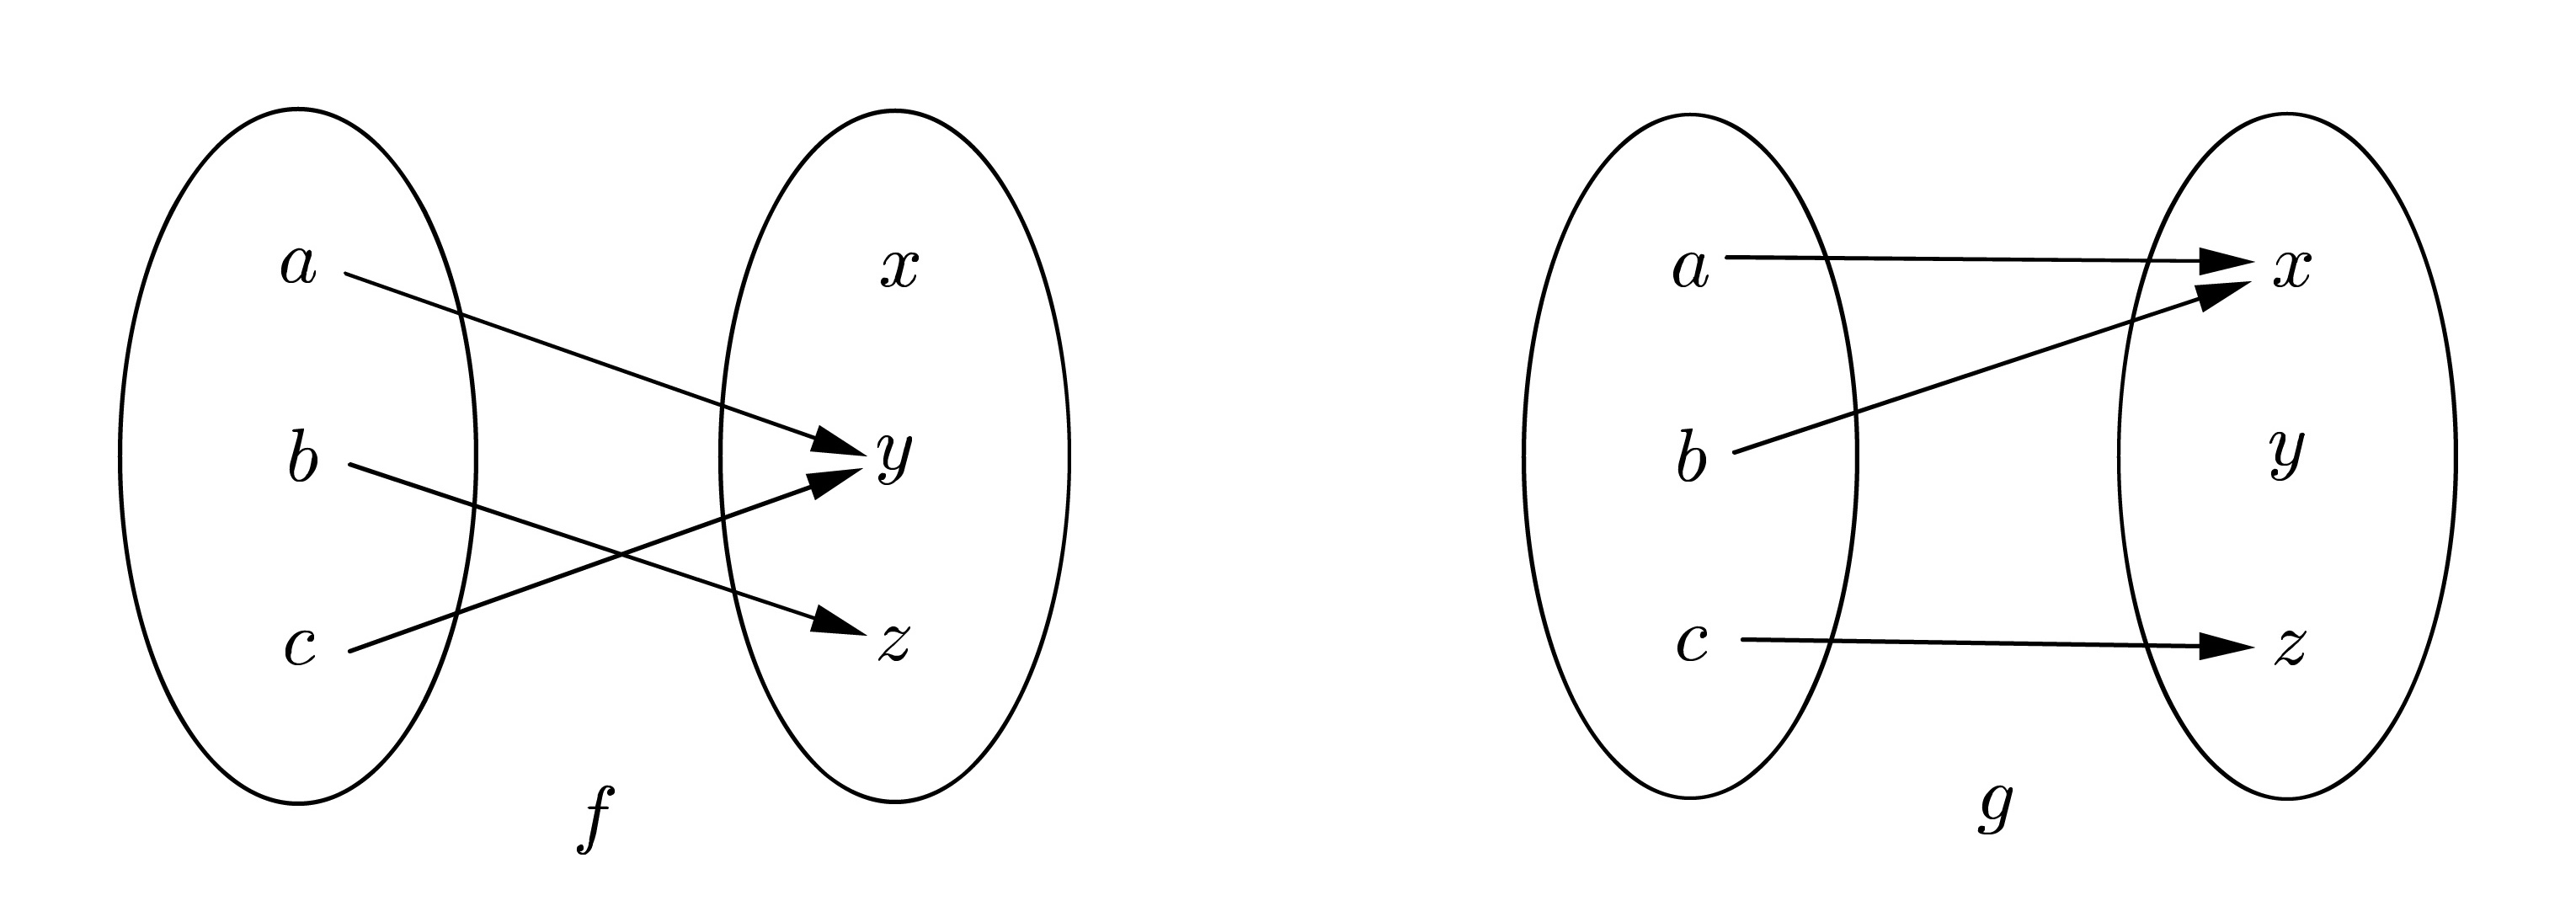
\includegraphics[width=.7\textwidth]{./images/cont1.jpg}
\end{figure}


The function $f$ is continuous since the inverse of each member of the topology $\tau^*$ on $Y$ is a member of the topology $\tau$ on $X$. The function $g$ is not continuous since $\{y,z\}\in \tau^*$ i.e. is an open subset of $Y$ but its inverse image $g^{-1}[\{y,z\}]=\{c\}$ is not an open subset of $X$ i.e. doesn't belong to $\tau$.
\end{example}

\begin{proposition}
A function $f:X \rightarrow Y$ is continuous if and only if the inverse image of every closed subset of $Y$ is a closed subset of $X$.
\end{proposition}
\begin{proof}
 Suppose $f:X\rightarrow Y$ is continuous, and $A$ a closed subset of $Y$. Then $A'$ is open, and so $f^{-1}(A')$ is open in $X$. But $f^{-1}[A']=(f^{-1}[A])'$; therefore $f^{-1}[A]$ is closed.\\
Conversely, assume $A$ closed in $Y$ implies $f^{-1}[A]$ closed in $X$. Let $G$ be an open subset of $Y$. Then $G'$ is closed in $Y$, and so $f^{-1}[G']=(f^{-1}[G])'$ is closed in $X$. Hence, $f^{-1}[G]$ is open and therefore $f$ is continuous.
\end{proof}

\begin{proposition}
Let the function $f:X\rightarrow Y$ and $g:Y\rightarrow Z$ be continuous maps. Then the composition function $g\circ f:X\rightarrow Z$ is also continuous.
\end{proposition}

\begin{proof}
Let $G$ be an open subset of $Z$. Then $g^{-1}[G]$ is open in $Y$ since $g$ is continuous. But $f$ is also a continuous, so $f^{-1}[g^{-1}[G]]$ is open in $X$. Now
$$ (g\circ f)^{-1}[G]=f^{-1}[g^{-1}[G]]$$
Thus, $(g\circ f)^{-1}[G]$ is open in $X$ for every open subset $G$ in $Z$. Therefore $g\circ f$ is a continuous map.

\end{proof}

\begin{theorem}[\textbf{The pasting lemma}]\label{pasting}
Let $X=A\cup B$, where $A$ and $B$ are closed in $X$. Let $f:A\rightarrow Y$ and $g:B\rightarrow Y$ be continuous. If $f(x)=g(x)$ for every $x\in A\cup B$, then $f$ \text{and} $g$ combine to give a continuous function $h:X\rightarrow Y$ defined by setting $h(x)=f(x)$ if $x\in A$ and $h(x)=g(x)$ if $x\in B$.
\end{theorem}
\begin{proof}
Let $C$ be a closed subset of $Y$. Now
$$h^{-1}(C)= f^{-1}(C)\cup g^{-1}(C),$$
by elementary set theory. Since $f$ is continuous, $f^{-1}(C)$ is closed in $A$ hence closed in $X$. Similarly, $g^{-1}(C)$ is closed in $B$ and therefore closed in $X$. Their union $h^{-1}(C)$ is thus closed in $X$.

\end{proof}

\section{Homeomorphism}

One major aspect of mathematics is how to find the correct notion of calling two things “equivalent.” In the theory of metric spaces\footnote{A metric on a non empty set is a function  $d: X\times X \rightarrow \mathbb{R}^+$ satisfying
\begin{enumerate}
  \item $d(x,y)\geq0$ and $d(x,x)=0$
  \item $d(x,y)=d(y,x), \forall x,y\in X$
  \item $d(x,z)\leq d(x,y)+d(y,z), \forall x,y,z\in X$
\end{enumerate}
The couple $(X,d)$ is called a metric space.}, the strongest possible such notion is called an isometry. That is, two metric spaces $X, Y$ with metrics $d_X, d_Y$ are called isometric if there exists a surjective function $f: X \to Y$ which preserves distance (i.e. $d_X(x,y) = d_Y(f(x), f(y))$ for all $x,y \in X,$ and the image $f(X)$ is all of $Y$). It is not hard to see that such functions are automatically both continuous and injective. The function $f$ is called an isometry.

Now we can call two metric spaces "the same" if they are isometric. Because we don't have distances in a topological space, the next best thing is a notion of equivalence based on continuity. This gives rise to the following definition.
\begin{definition}[\textbf{Mobius}]
Let $X$ and $Y$ be topological spaces; let $f : X\rightarrow Y$ be a bijection. If both the function $f$ and the inverse function
$$f^{-1}: Y\rightarrow X$$
are continuous, then f is called a homeomorphism.
\end{definition}

The condition that $f^{-1}$ be continuous says that for each open set $U$ of $X$, the inverse image of $U$ under the map $f^{-1}: Y\rightarrow X$ is open in $Y$ . But the inverse image of $U$ under the map $f^{-1}$ is the same as the image of $U$ under the map $f$ . So another way to define a homeomorphism is to say that it is a bijective
correspondence $f : X\rightarrow Y$ such that $f(U)$ is open if and only if $U$ is open.
